\tikzstyle{field}=[rectangle,draw=black,line width=1pt,align=center,font=\footnotesize,minimum height=1cm]
\linespread{0.8}

\scalebox{.66}{
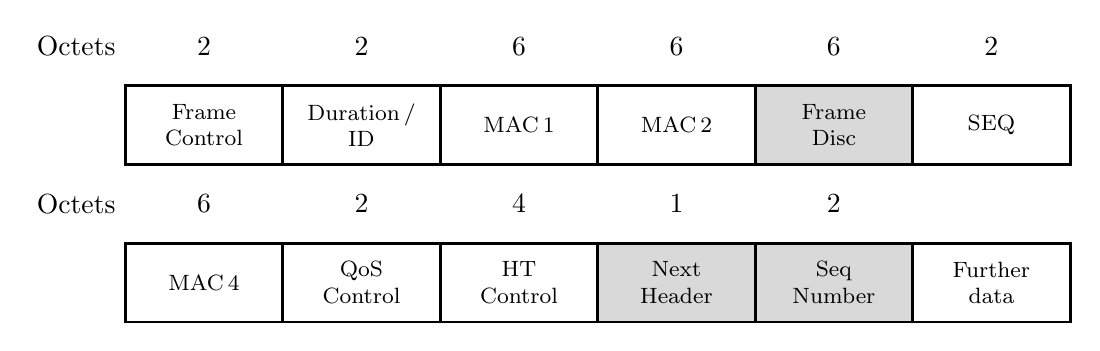
\begin{tikzpicture}[>=latex]
	%\draw (0,0) rectangle (2,1);
	\node[field,minimum width=2cm] at (0,0) {Frame\\Control};
	\node[field,minimum width=2cm] at (2,0) {Duration\,/\\ID};
	\node[field,minimum width=2cm] at (4,0) {MAC\,1};
	\node[field,minimum width=2cm] at (6,0) {MAC\,2};
	\node[field,minimum width=2cm,fill=gray!30] at (8,0) {Frame\\Disc};
	\node[field,minimum width=2cm] at (10,0) {SEQ};


	\node[field,minimum width=2cm] at (0,-2) {MAC\,4};
	\node[field,minimum width=2cm] at (2,-2) {QoS\\Control};
	\node[field,minimum width=2cm] at (4,-2) {HT\\Control};
	\node[field,minimum width=2cm,fill=gray!30] at (6,-2) {Next\\Header};
	\node[field,minimum width=2cm,fill=gray!30] at (8,-2) {Seq\\Number};
	\node[field,minimum width=2cm] at (10,-2) {Further\\data};

	% Bits
	\node[left] at (-1,1) {Octets};
	\node at (0,1) {2};
	\node at (2,1) {2};
	\node at (4,1) {6};
	\node at (6,1) {6};
	\node at (8,1) {6};
	\node at (10,1) {2};
	
	\node[left] at (-1,-1) {Octets};
	\node at (0,-1) {6};
	\node at (2,-1) {2};
	\node at (4,-1) {4};
	\node at (6,-1) {1};
	\node at (8,-1) {2};

\end{tikzpicture}
}
